\documentclass{article}
\usepackage{amsmath}

\usepackage{full page}  % make the margins somewhat smaller than the default

\usepackage{listings}  %  needed for source code listings
\usepackage{color}
\usepackage{hyperref}
\usepackage{graphicx}
\usepackage{caption}
\usepackage{subcaption}
\usepackage{float}

\graphicspath{ {images/} }

\definecolor{javared}{rgb}{0.7,0,0} % for strings
\definecolor{javagreen}{rgb}{0.25,0.6,0.35} % comments
\definecolor{javapurple}{rgb}{0.55,0,0.40} % keywords
\definecolor{javadocblue}{rgb}{0.25,0.35,0.85} % javadoc
 
\lstset{language=Java,
basicstyle=\ttfamily,
keywordstyle=\color{javapurple}\bfseries,
stringstyle=\color{javared},
commentstyle=\color{javagreen},
morecomment=[s][\color{javadocblue}]{/**}{*/},
numbers=left,
numberstyle=\tiny\color{black},
stepnumber=2,
numbersep=10pt,
tabsize=2,
showspaces=false,
showstringspaces=false,
frame=shadowbox,
numbers=left
} 

% set the document title, author, and date here.
%  once set, the \maketitle command (within the document)
%  will display them nicely
\title{AI Assignment 5 - Constraint Satisfaction Problem}
\author{Tianyuan Zhang}

\begin{document}
\maketitle

\section{Introduction}
Constraint satisfaction problems are a kind of problem that can be described as a series of variables, domains, and constraints. CPS an important method in AI field as it can use a standard model to solve a lot of different problems.

\section{The Design of CSP Solver}
\subsection{Basic Idea}
In a typical constraint satisfaction problem, the problem can be represented as variables, values and constraints, as following:
$$X = \{X_1, ..., X_n\}$$
$$D = \{D_1, ..., D_n\}$$
$$C = \{C_1, ..., C_m\}$$
where $X$ represents the variable, $D$ represents the domain for the corresponding variable, and $C$ represents the constraint for each pair of variables. The goal is to assign each variable a value from their corresponding domain while satisfying all the constraints in $C$.

\subsection{CSP Class Design}
The abstract class $CSP$ contains all the needed members and methods for solving CSP.
\subsubsection{Pair}
There is a subclass under the $CSP$ class which names $Pair$. This class is for store a pair of variable and also define the equal, compare and hashcode for the $Pair$ type.
\begin{lstlisting}
	//class for Pair, custom equal and hashcode
	public class Pair implements Comparable<Pair>{
		protected int x;
		protected int y;
		
		public Pair(int _a, int _b){
			x = _a; y = _b;
		}
		
		@Override
	    public boolean equals(final Object o) {
	        if (this == o) return true;
	        
	        if (!(o instanceof Pair)) return false;

	        final Pair pair = (Pair) o;
	        if (x != pair.x) return false;
	        if (y != pair.y) return false;
	        return true;
	    }

	    @Override
	    public int hashCode() {
	        int result = x;
	        result = 31 * result + y;
	        return result;
	    }
	    
	    @Override
		public int compareTo(Pair o) {
			return (int) Math.signum(- this.x + o.x);
		}
	    
	    @Override
	    public String toString(){
	    	return '[' + Integer.toString(x) + ',' + Integer.toString(y) + ']';
	    }
	}
\end{lstlisting}

\subsubsection{members}
There are several members in the $CSP$ class and here is the explanation for each of them.
\begin{lstlisting}
	protected int[] assignment;
	protected int varNum;
	protected HashMap<Pair, HashSet<Pair>> constraint;
	protected HashMap<Integer, HashSet<Integer>> domain;
	protected HashMap<Integer, HashSet<Integer>> domainOriginal;
	protected HashMap<Integer, HashSet<Integer>> adjList;
	protected HashSet<Pair> adjPairList;
	private boolean MRV = false;
	private boolean LCV = false;
	private boolean AC3 = false;
\end{lstlisting}
\begin{flushleft}
The $assignment$ array stores the value for each variable. A value of -1 means no value assigned to that variable.

The $varNum$ means the number of variables

The $constraint$ stores the allowable value pair for the variable pair.

The $domain$ stores allowable values for each variable.

The $domainOriginal$ stores the original domain of variables, as the $domain$ will keep changing during the computing process.

The $adjList$ stores variable as key and its adjacent variables as map values.

The $adjList$ store every pair of variables that is adjacent.

The $MRV$, $LCV$, and $AC3$ stores whether the corresponding method needs to be applied or not.
\end{flushleft}

\subsubsection{dfs}
The method $dfs()$ is a depth-first search method that will try every possible combination for $assignment$ as long as the values satisfy the $constraints$.
\begin{lstlisting}
	public boolean dfs(){	
		int var = nextVar();
		if(var == -1) return true;
		List<Integer> values = getValues(var);
		HashMap<Integer, HashSet<Integer>> dupDomain;
		for(Integer val : values){
			if(checkConsistent(var, val)){
				//try the assignment and domain
				assignment[var] = val;
				dupDomain = domainCopy(domain);
				domain.get(var).clear();
				domain.get(var).add(val);
				if(AC3) ac_3();
				if(dfs()) return true;
				
				//recover the assignment and the domain
				assignment[var] = -1;
				domain.clear();
				domain = dupDomain;
			}
		}
		
		return false;
	}
\end{lstlisting}

\subsubsection{checkConsistent}
The method $checkConsistent$ will try a variable a value and check if there is any confliction occur in the $assignment$. 
\begin{lstlisting}
private boolean checkConsistent(int var, int val){
	for(int i = 0; i < varNum; i++){
		if(var == i || assignment[i] == -1) continue;
		Pair varPair = new Pair(var, i);
		Pair valPair = new Pair(val, assignment[i]);
		if(constraint.containsKey(varPair)){
			if(!constraint.get(varPair).contains(valPair))
				return false;
		}
	}	
	return true;
}
\end{lstlisting}

\subsubsection{nextVar(MRV)}
The method $nextVar()$ will return the next variable that needs to be estimated. If the member $MRV$ is false, then this method will simply choose the first next unestimated variable. Otherwise, MRV method will be applied and choose the next variable with the least domain size.
\begin{lstlisting}
	int nextVar(){
		if(MRV){
			int minDomainSize = Integer.MAX_VALUE;
			int minVar = -1;
			for(int i = 0; i < varNum; i++){
				if(assignment[i] == -1 && domain.get(i).size() < minDomainSize){
					minDomainSize = domain.get(i).size();
					minVar = i;
				}
			}
			return minVar;
		} else{
			for(int i = 0; i < varNum; i++)
				if(assignment[i] == -1)
					return i;
		}
		return -1;
	}
\end{lstlisting}

\subsubsection{getValues(LCV)}
The method $getValues$ will return a list of values for the $dfs$ method to choose for the current estimating variable. If member $LCV$ is false, then this method simply returns the list of values from the domain without reordering. Otherwise, this method will estimate the confliction arisen by the value and return a list of values, with least confliction value in the front.
\begin{lstlisting}
	private List<Integer> getValues(int var){
		List<Integer> values = new ArrayList<>();
		if(LCV){
			PriorityQueue<Pair> q = new PriorityQueue<Pair>();
			HashSet<Integer> varDomain = domain.get(var);
			for(int val : varDomain){
				int ruledSize = 0;
				assignment[var] = val;
				for(int adjVar : adjList.get(var)){
					if(assignment[adjVar] == -1 &&
							domain.get(adjVar).contains(val))
						ruledSize++;
				}
				assignment[var] = -1;
				Pair pair = new Pair(ruledSize, val);
				q.add(pair);
			}
			
			while(!q.isEmpty())
				values.add(q.poll().y);
		}
		else{
			for(int val : domain.get(var))
				values.add(val);
		}
		return values;
	}
\end{lstlisting}

\subsubsection{AC3}
The method $ac_3()$ is the method to apply AC3 algorithms for the current assignment. Basically, this method will remove every conflicted value from the domain for the unestimated variable according to the estimated variables value. Method $removeInconVal$ will be called to check if a domain of a variable has been changed. 
\begin{lstlisting}
	private void ac_3(){
		Queue<Pair> q = new LinkedList<Pair>();
		for(Pair pair : adjPairList)
			q.add(pair);
		while(!q.isEmpty()){
			Pair cur = q.poll();
			if(assignment[cur.x] != -1) continue;
			if(removeInconVal(cur.x, cur.y)){
				for(int var : adjList.get(cur.x)){
					if(var != cur.y && assignment[var] != -1)
						q.add(new Pair(var, cur.x));
				}
			}
		}
	}
	
	private boolean removeInconVal(int var1, int var2){
		boolean removed = false;
		boolean found = false;
		Pair varPair = new Pair(var1, var2);
		if(!constraint.containsKey(varPair)) return false;
		HashSet<Pair> cur = constraint.get(varPair);
		HashSet<Integer> var1Domain = new HashSet<Integer>();
		var1Domain.addAll(domain.get(var1));
		for(int val1 : var1Domain){
			for(int val2 : domain.get(var2)){
				if(cur.contains(new Pair(val1, val2))){
					found = true;
					break;
				}
			}
			if(found == false){
				domain.get(var1).remove(val1);
				removed = true;
			}
			found = false;
		}
		return removed;
	}
\end{lstlisting}

\section{Map Coloring Problem}
The Map Coloring Problem is a classic problem that can be modeled as a constraint satisfied problem. The goal is to assign each city a color in the map so that no adjacent cities share the same color.
\subsection{Convert to CSP Model}
It is quite straightforward to convert map coloring problem into a CSP. We can assign each city a unique integer and assign each color a unique integer. Then we can use an array $assignment$ to represent the result, where the index of the array indicates the city and the value of that index in the array represent which color is assigned to this city. Also, $adjList$ and $adjPairList$ is created according to the map of cities. 

\subsection{buildDomain}
Thie method will build the domain according to the input. It is quite simple as each city have the same domain - all the possible colors.
\begin{lstlisting}
	private HashMap<Integer, HashSet<Integer>> buildDomain(int cityNum, int colorNum){
		HashMap<Integer, HashSet<Integer>> builder = new HashMap<>();
		for(int i = 0; i < cityNum; i++){
			builder.put(i, new HashSet<Integer>());
			for(int j = 0; j < colorNum; j++)
				builder.get(i).add(j);
		}
		return builder;
	}
\end{lstlisting}

\subsection{buildConstraint}
The method $buildConstraint$ will build the constraint according to the input. For each possible adjacent cities, the allowable values pair is the pair that assigns each city a different color.
\begin{lstlisting}
	private HashMap<Pair, HashSet<Pair>> buildConstraint(){
		HashMap<Pair, HashSet<Pair>> builder = new HashMap<>();
		for(Pair cityPair : adjPairList){
			HashSet<Pair> allPair = getAllColorPair(cityPair);
			builder.put(cityPair, allPair);
		}
		return builder;
	}
	
	private HashSet<Pair> getAllColorPair(Pair cityPair){
		HashSet<Pair> allPair = new HashSet<>();
		HashSet<Integer> var1Domain = domain.get(cityPair.x);
		HashSet<Integer> var2Domain = domain.get(cityPair.y);
		for(Integer color1 : var1Domain){
			for(Integer color2 : var2Domain){
				if(color1 == color2) continue;
				Pair pair = new Pair(color1, color2);
				allPair.add(pair);
			}
		}
		return allPair;
	}
\end{lstlisting}

\subsection{Result}
For the result part, I tried the given test case and my implementation gives me the expected result. I also tried to apply MRV, LCV or AC3 and all of them gives me the correct result, though the result is not exact the same. I will use the Circuit Board Problem to analyze the performance, so this result is only showing the correctness of this implementation.
\begin{lstlisting}
MRV:false LCV:false AC3:false
WA->Red NT->Blue SA->Green Q->Red NSW->Blue V->Red T->Red 
Run Time: 1 ms

MRV:true LCV:false AC3:false
WA->Red NT->Blue SA->Green Q->Red NSW->Blue V->Red T->Red 
Run Time: 0 ms

MRV:false LCV:true AC3:false
WA->Red NT->Green SA->Blue Q->Red NSW->Green V->Red T->Red 
Run Time: 2 ms

MRV:false LCV:false AC3:true
WA->Red NT->Blue SA->Green Q->Red NSW->Blue V->Red T->Red 
Run Time: 2 ms

\end{lstlisting}

\section{Circuit Board Problem}
The Circuit Board Problem is another problem that can be generalized as a Constraint Satisfied Problem. The goal for this problem is to compute the arrangement of each component on the circuit board, given the board's size and each component's size.
\subsection{Convert to CSP Model}
The way to convert a Circuit Board Problem to a CSP model is not that straightforward as the map coloring one. We can still assign each component a unique integer to represent each of them. However, when it comes to the value part, we need to convert the coordinate of components top-left corner to a single integer. The way I used in my implementation is the same as converting 2D array into 1D array, that $1D\_idx = 2D.x * width + 2D.y$. Then we can represent each position in the board by a unique integer.

\subsection{buildDomain}
This method will build domain for each component given their size and the board's size. The only constraint that need to be applied here is that the component can not go outside the board.
\begin{lstlisting}
	private HashMap<Integer, HashSet<Integer>> buildDomain(){
		HashMap<Integer, HashSet<Integer>> builder = new HashMap<>();
		for(Pair comp : components){
			int idx = comp2Idx.get(comp);
			builder.put(idx, new HashSet<>());
			for(int x = 0; x + comp.x - 1 < width; x++){
				for(int y = 0; y + comp.y - 1 < height; y++){
					builder.get(idx).add(y * width + x);
				}
			}
		}
		return builder;
	}
\end{lstlisting}

\subsection{buildConstraint}
This method will build constraint for each pair of variables. For this circuit board problem, the constraint is that two components cannot overlap each other. The way to check if two components overlap is to get their center point first. Then these two components are overlapped only if their center point's horizontal distance is less than half of their width sum and the vertical distance is less than half of their height sum.
\begin{lstlisting}
	private HashMap<Pair, HashSet<Pair>> buildConstraint(){
		HashMap<Pair, HashSet<Pair>> builder = new HashMap<>();
		for(Pair comp1 : components){
			for(Pair comp2 : components){
				if(comp1.equals(comp2)) continue;
				Pair varPair = new Pair(comp2Idx.get(comp1), comp2Idx.get(comp2));
				HashSet<Pair> varConstraints = getPairConstraint(comp1, comp2);
				builder.put(varPair, varConstraints);
			}
		}
		return builder;
	}
	
	private HashSet<Pair> getPairConstraint(Pair comp1, Pair comp2){
		int compIdx1 = comp2Idx.get(comp1);
		int compIdx2 = comp2Idx.get(comp2);
		HashSet<Pair> pairConstraints = new HashSet<Pair>();
		for(Integer domain1 : domain.get(compIdx1)){
			for(Integer domain2 : domain.get(compIdx2)){
				int x1 = domain1 % width;
				int y1 = domain1 / width;
				double x1_mid = (double)(x1) + (double)(comp1.x) / 2.0;
				double y1_mid = (double)(y1) + (double)(comp1.y) / 2.0;
				int x2 = domain2 % width;
				int y2 = domain2 / width;
				double x2_mid = (double)(x2) + (double)(comp2.x) / 2.0;
				double y2_mid = (double)(y2) + (double)(comp2.y) / 2.0;
				if(Math.abs(x1_mid - x2_mid) >=  (double)(comp1.x + comp2.x) / 2.0 
					|| Math.abs(y1_mid - y2_mid) >= (double)(comp1.y + comp2.y) / 2.0)
					pairConstraints.add(new Pair(domain1, domain2));
			}
		}
		return pairConstraints;
	}
\end{lstlisting}

\subsection{Result}
As Circuit Board Problem is easier to think of a large scale example, I test the performance difference here.

\subsubsection{Given Sample}
The sample that is given by the instruction is very simple. Even the brute force method provide a 1 ms run time. The following is the result.
\begin{lstlisting}
MRV:false LCV:false AC3:false
[A, A, A, B, B, B, B, B, C, C]
[A, A, A, B, B, B, B, B, C, C]
[D, D, D, D, D, D, D, ., C, C]
Run Time: 1 ms

MRV:true LCV:false AC3:false
[C, C, B, B, B, B, B, A, A, A]
[C, C, B, B, B, B, B, A, A, A]
[C, C, D, D, D, D, D, D, D, .]
Run Time: 0 ms

MRV:false LCV:true AC3:false
[A, A, A, B, B, B, B, B, C, C]
[A, A, A, B, B, B, B, B, C, C]
[., D, D, D, D, D, D, D, C, C]
Run Time: 4 ms

MRV:false LCV:false AC3:true
[A, A, A, B, B, B, B, B, C, C]
[A, A, A, B, B, B, B, B, C, C]
[D, D, D, D, D, D, D, ., C, C]
Run Time: 2 ms
\end{lstlisting}

\subsubsection{Large Scale Sample - Tight}
To better test the performance difference, I create a large scale sample.This is a tight sample, as there is not much space left after arranging each component on the board. The board size becomes 30*6 and each component's size is as follows:
\begin{lstlisting}
	List<List<Integer>> components = new ArrayList<>();
	components.add(Arrays.asList(10,5));
	components.add(Arrays.asList(15,7));
	components.add(Arrays.asList(5,1));
	components.add(Arrays.asList(5,4));
	components.add(Arrays.asList(20,1));
	components.add(Arrays.asList(25,1));
	components.add(Arrays.asList(3,7));
	components.add(Arrays.asList(2,8));
	int width = 30;
	int height = 9;
\end{lstlisting}

Then I tried a different combination of MRV, LCV and AC3. All of them give me reasonable answer though they are not the same. The following is one of the results generated by the code.
 
\begin{figure}[H]
\centering
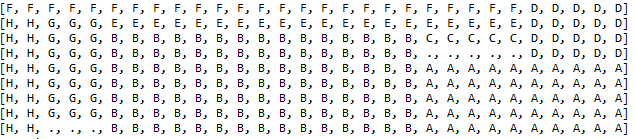
\includegraphics[width=\linewidth]{TightResult}
\caption{Result - Tight}
\end{figure}

And the following is the run time and the corresponding bar graph. It is clear that AC3 provide a huge performance improvement, which is as expected because in AC3 we delete all the conflict values in domain and thus the DFS tree will be able to prevent searching a lot of branches. The LCV method provides a reasonable performance improvement as it reorders the values. However as the recorder also cost a lot running time, this method would waste a lot of time on a small scale problem. The interesting part about the test is that MRV spent more time than the normal method. I think the reason is that MRV is just a method to reorder the variable. As in circuit board problem each component has a lot of possible values, reordering variables may not have a huge impact as domain reduction, like LCV or AC3.
\begin{lstlisting}
MRV:false LCV:false AC3:false
Run Time: 570 ms

MRV:true LCV:false AC3:false
Run Time: 1624 ms

MRV:false LCV:true AC3:false
Run Time: 448 ms

MRV:false LCV:false AC3:true
Run Time: 12 ms

MRV:true LCV:true AC3:false
Run Time: 1450 ms

MRV:true LCV:false AC3:true
Run Time: 40 ms

MRV:false LCV:true AC3:true
Run Time: 14 ms

MRV:true LCV:true AC3:true
Run Time: 28 ms
\end{lstlisting}
\begin{figure}[H]
\centering
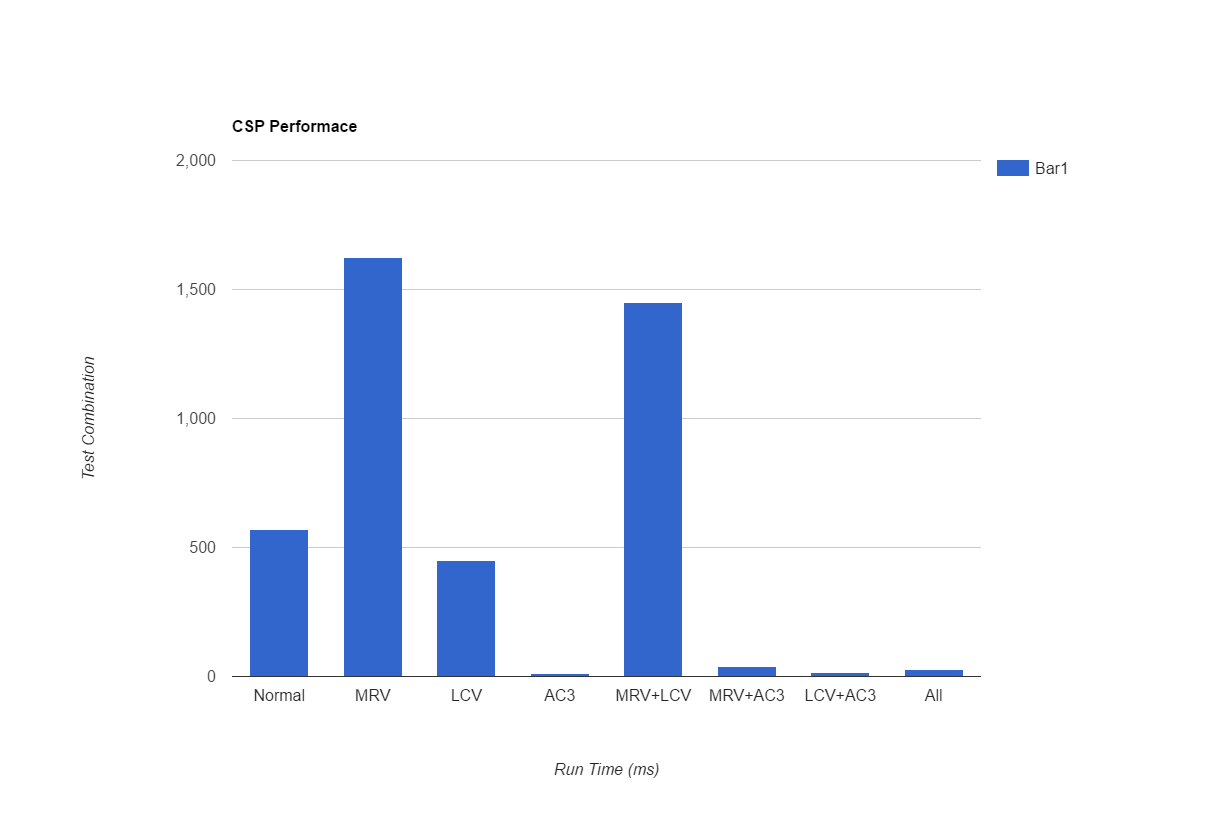
\includegraphics[width=\linewidth]{TightBarGraph}
\caption{Bar Graph for Tight Sample}
\end{figure}

\subsubsection{Large Scale Sample - Sparse}
Then I tried another sample, the only different from the previous test sample is that I tried fewer components here, which mean there will be more space after arranging all the components on the board. The following is one of the results generated by the code.

\begin{figure}[H]
\centering
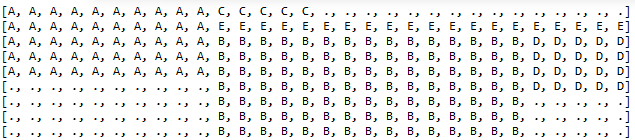
\includegraphics[width=\linewidth]{SparseResult}
\caption{Result - Sparse}
\end{figure}

And the following is the run time and the corresponding bar graph. Clearly under the sparse condition MRV provide a slight performance improvement while LCV and AC3 slow down the computation. I think the reason is that as a result is sparse, the domain shrink very slowly and LCV and AC3 have no significant effect on improving the performance. While on the MRV side, the variables' reordering gives the chance to approach the final result in a shorter time.
\begin{lstlisting}
MRV:false LCV:false AC3:false
Run Time: 6 ms

MRV:true LCV:false AC3:false
Run Time: 5 ms

MRV:false LCV:true AC3:false
Run Time: 14 ms

MRV:false LCV:false AC3:true
Run Time: 9 ms

MRV:true LCV:true AC3:false
Run Time: 14 ms

MRV:true LCV:false AC3:true
Run Time: 11 ms

MRV:false LCV:true AC3:true
Run Time: 13 ms

MRV:true LCV:true AC3:true
Run Time: 5 ms
\end{lstlisting}

\begin{figure}[H]
\centering
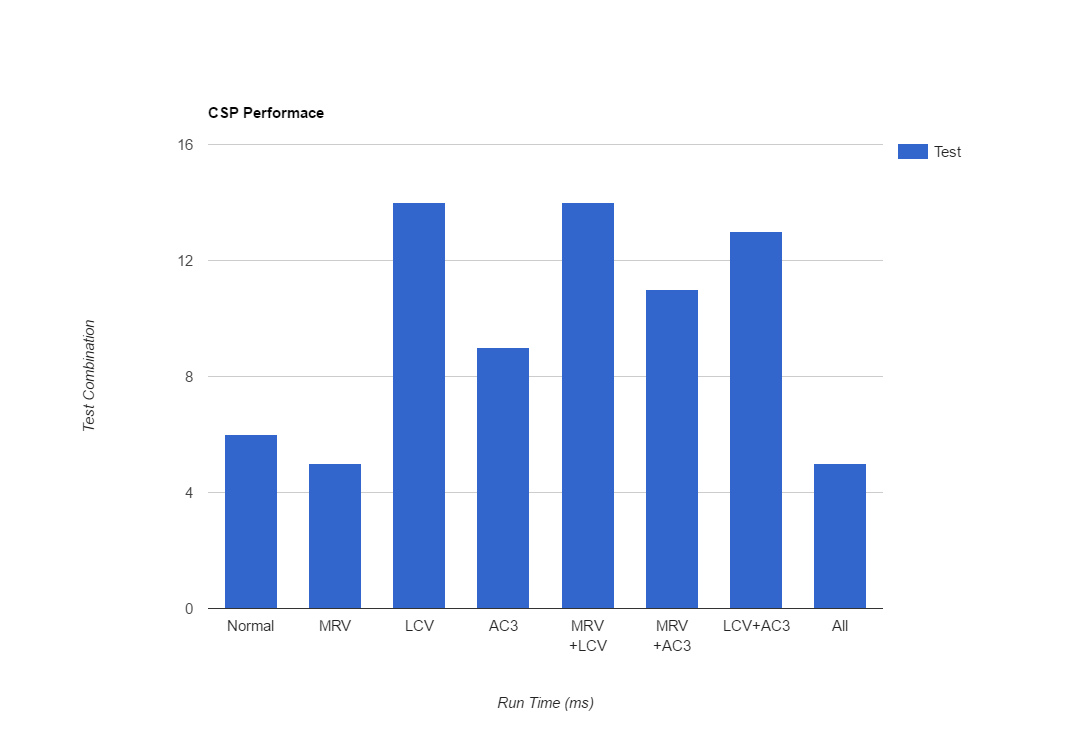
\includegraphics[width=\linewidth]{SparseBarGraph}
\caption{Bar Graph for Sparse Sample}
\end{figure}

\section{Summary}
From the tests I made above, I found that for the extremely small scale problem, the normal CSP method would be enough as any other computation will add the computing time to the system. For a medium scale problem, I may want to open the MRV or LCV method as they can provide a reasonable performance improvement. And for large scale problem, I would choose the LCV + AC3 method as this two method provides significant performance improvement by diving into possible correct branch quicker and shrinking the domain at a faster pace.

\end{document}